\chapter{Countermeasures}
\label{countermeasures}
In this chapter, we describe the various strategies that the operator can put in place to strengthen the traffic of a vulnerable LoRa network. The goal is to reduce the amount of exposed ED recognized by PIVOT, modifying the devices' configuration to avoid being detected again by the system. From a technical point of view, the administrator should reduce the values of \textit{NoDD} (Number of Detected Devices) and the  \textit{PoDD} (Percentage of Detected Devices) metrics. NoDD and PoDD are directly proportional, but they can refer to different contexts. Generally speaking, NoDD is designed to describe small networks, where devices have more predictable behavior. PoDD describes better those situations where the number of devices is much greater. For example, given a network with twelve vulnerable devices out of a total of twenty active ones, we have the following metrics \(\ NoUD = 20 \) and \(\ NoDD = 12 \), from which we derive \(\ PoDD = \frac{NoDD}{NoUD} = 0.6 \). The output of this metric could indicate a critical status of the network. However, if the operator compares the high value of PoDD to the lower value of NoDD, it recognizes that it has to modify the behavior of only twelve devices. It might be a more alarming circumstances if \(\ PoDD = 0.6 \) but \(\ NoUD = 1000 \)!

\vspace{5mm} %5mm vertical space

PIVOT alters the operator when a device has a too predictable behavior that could expose it to unauthorized information disclosure, such as the association of the \textit{DevAddr} identifiers to the global \textit{DevEUI} address. The strategy behind the PIVOT detection algorithm is the \textit{pattern-matching}. Therefore, the positivity of the outcome is closely related to the periodic pattern of the target device. This prerequisite implies that all countermeasures that do not alter the regularity in the ED flow prove to be ineffective. Our challenge is to change the pattern of the exposed device without compromising the purpose for which it is created.  For example, if the target ED is an industrial pressure sensor designed to periodically send updates to the server, the operator should keep in mind that changing the behavior of the device could alter this basic functioning. Since we want to avoid that eavesdroppers can extrapolate the devices' patterns from analyzing the LoRa flow, the solutions we will describe are related to the family of the \textit{pattern detection} countermeasures.

\vspace{5mm}

The first strategy we present is the addition of the so-called dummy packets to EDs transmissions. In the LoRaWAN frame, only the payload is encrypted, making these dummy messages indistinguishable from those containing the information. On the other side, the application server, provided with a packet filter, can distinguish real data from fake ones. 
Although several studies \cite{5283315} show the effectiveness of this technique, we want to point out several disadvantages that lead us to exclude it as a final solution. First, this mechanism impacts performance, reducing channel availability. Moreover, the transmission of additional packets requires more energy than desired, inevitably reducing the lifetime of the ED. A implication that goes against the principles of LPWANs, such as LoRaWAN, designed with the principle to ensure the long duration of battery-operated devices. Finally, increasing the transition rate of the endpoints is a choice subject to various physical constraints. Indeed, as shown in figure \ref{fig:duty_cycle}, EDs can occupy the channel for a limited portion of time, called  \textit{duty cycle}. It is commonly set to 1\%, or 1-time unit every 100-time units \cite{8030482}.

\vspace{3mm}
\begin{figure}[H]
    \centering
    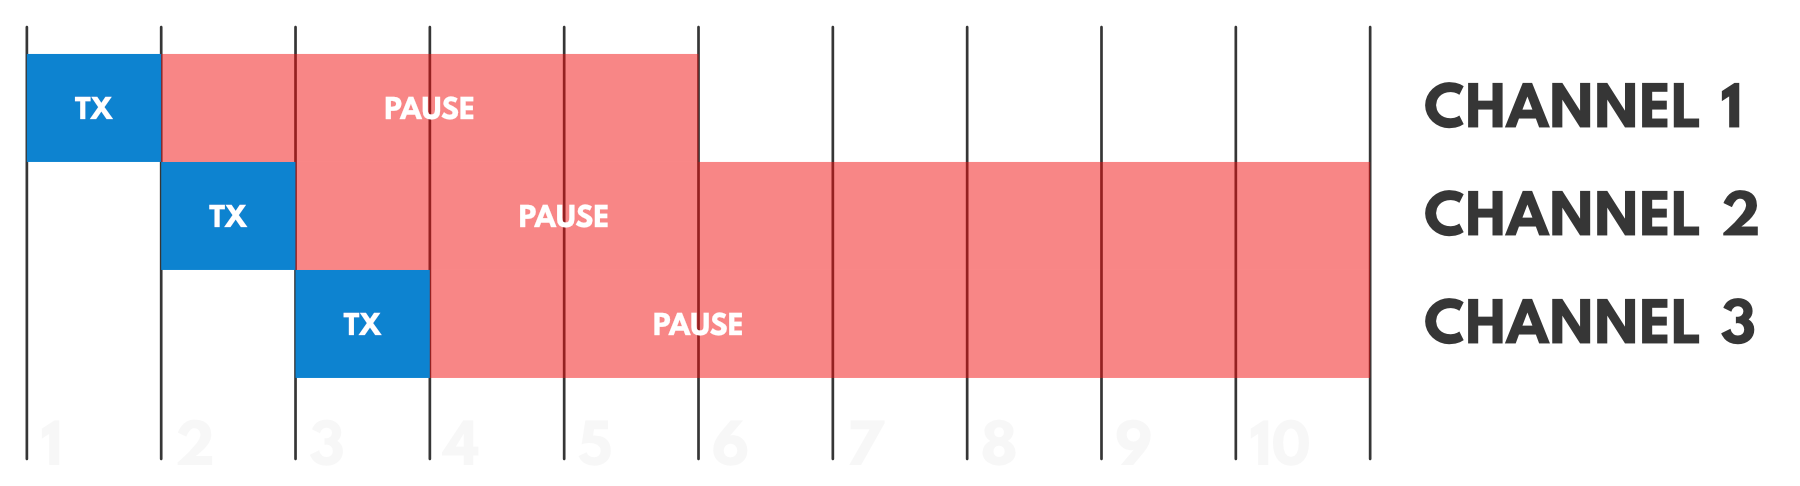
\includegraphics[width=0.7\linewidth]{images/countermeasures/duty_cycle.png}
    \caption{The duty cycle of LoRaWAN}
    \label{fig:duty_cycle}
\end{figure}
\vspace{3mm}

In this work, we go deeper. As shown in figure \ref{fig:flow}, rather than altering traffic by adding new data to the network, we propose to hide the periodic behavior of devices by changing the flow generated by them. In this way, we don't add irrelevant data within the network, preserving the performance and costs required. 

\vspace{3mm}
\begin{figure}[H]
    \centering
    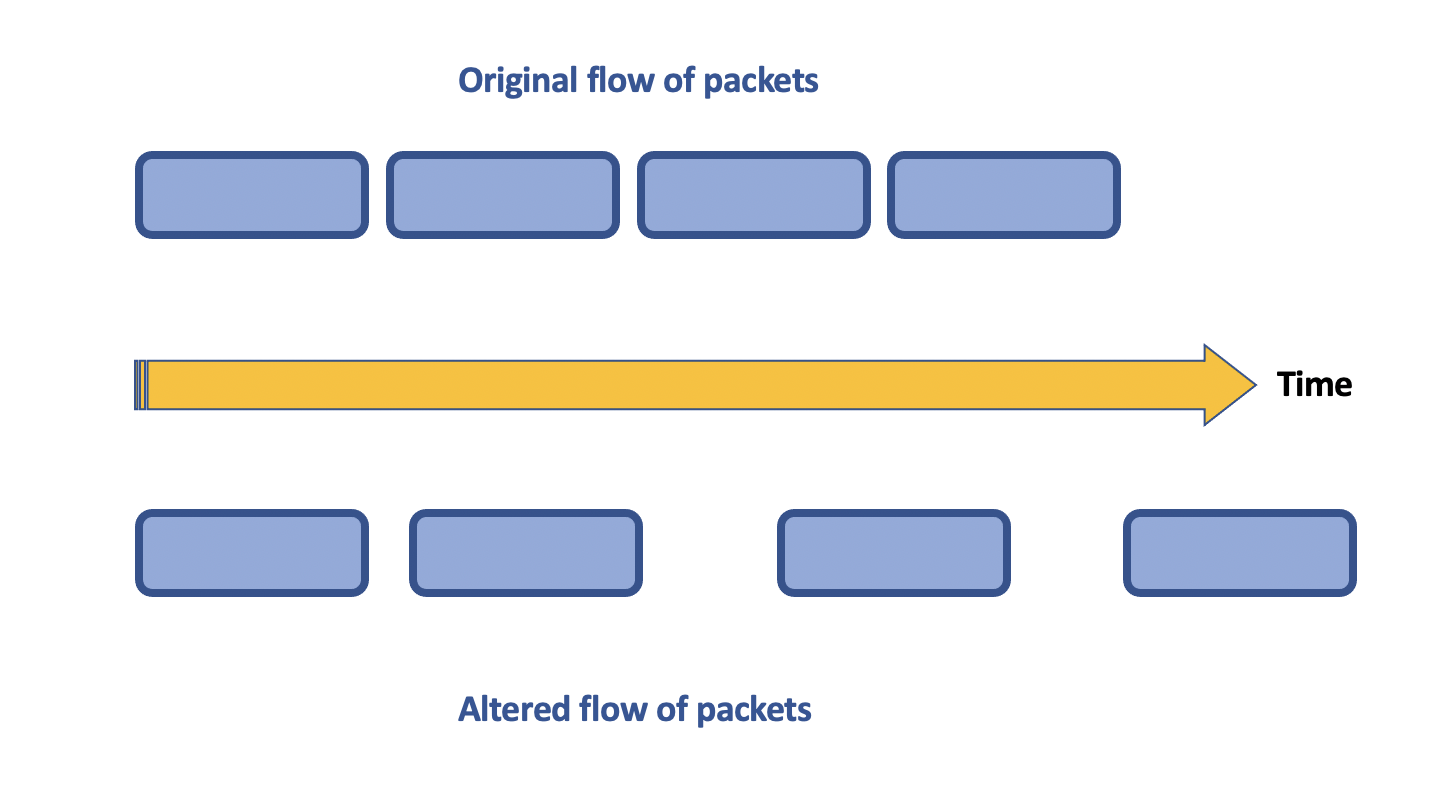
\includegraphics[width=0.7\linewidth]{images/countermeasures/flow.png}
    \caption{The altered flow}
    \label{fig:flow}
\end{figure}
\vspace{3mm}

A basic approach is to regularize the flow by requiring endpoints to send packets following the same frequencies. Covering the different EDs' patterns, the behaviors of the various devices are indistinguishable. But it is not suitable for all types of applications. Indeed, many scenarios, such as alarming systems, require a fast response, and following a forced behavior than required could be a very restrictive limitation. Made these considerations, we propose to add a \textit{random} delay before sending each packet. When the delay is high enough, the correlation between the device and its pattern is hidden. In detail, let be \(\ P \) the pattern as defined in Chapter \ref{pivot}:

\[\ P = \{ s_{1}, ..., s_{n} \} \]

And the let be \(\ d_{i} \) the randomly generated delay to add to each segment \(\ s_{i} \), then the we define the new pattern \(\ P' \) as:

\[\ P' = \{ s_{1} + d_{1}, ..., s_{n} + d_{n} \} \]

such that 
\[\ P \not\equiv P' \] 
for each \(\ d_{i} \) chosen.

\vspace{5mm}

The required delay can be extracted from a \textit{pseudo-random} number sampling, a procedure for generating numbers distributed according to a given \textit{probability distribution}. A well know pseudo-random number sampling method is the inverse transform sampling, which produces instances using the Cumulative Distribution Function (CDF) \(\ F_{X} \) of the random variable \(\ X \). The function \(\ F_{X} \) takes as input some value \(\ x \) outputs the probability of obtaining \(\ X \leq x \). 
\[\ F_{X}(x) = P(X \leq x) = p \]
The inverse transform sampling uses the inverse of CFD. The \(\ F_{X}^{-1} \) takes \(\ p \) as input and returns \(\ x \), where \(\ p \) is uniformly distributed. With this method, we can sample from any \(\ F_{X} \) if \(\ F_{X}^{-1}  \) is known. We need just to take values \(\ u \sim U(0,1) \) and then, through \(\ F_{X}^{-1}  \), obtain \(\ x \)'s.
\[\ F_{X}^{-1}(u) = x \]

\subsubsection{The exponential distribution}
Our idea is to simulate a random variable \(\ X \) that follows the \textit{exponential} distribution with mean \(\ \lambda \) i.e. \(\ X \sim Exp(\lambda) \). In queueing theory, this distribution lends itself well to modeling customer interarrival times or service times for several reasons \cite{QUEUING_THEORY}. First, the exponential function is a strictly decreasing function of \(\ t \), meaning that after arrival has occurred, the amount of waiting time until the next arrival is more likely to be small than large. Second, the exponential distribution is memoryless. This property implies that the time until the next arrival doesn't depend on the time that has already passed, preventing the adversary to extrapolate information about the behavior of the devices by analyzing their past transmissions. Specifically, if an adversary observes a packet after time \(\ t_1 \) and wants to calculate the probability of the next packet arriving after \(\ t_2 = \Delta t + t_1 \), the memorylessness property ensures that:
\[\ P(X>t_1+\Delta t \,|\, X>t_1) = P(X>\Delta t) \]

\vspace{3mm}
\begin{figure}[H]
    \centering
     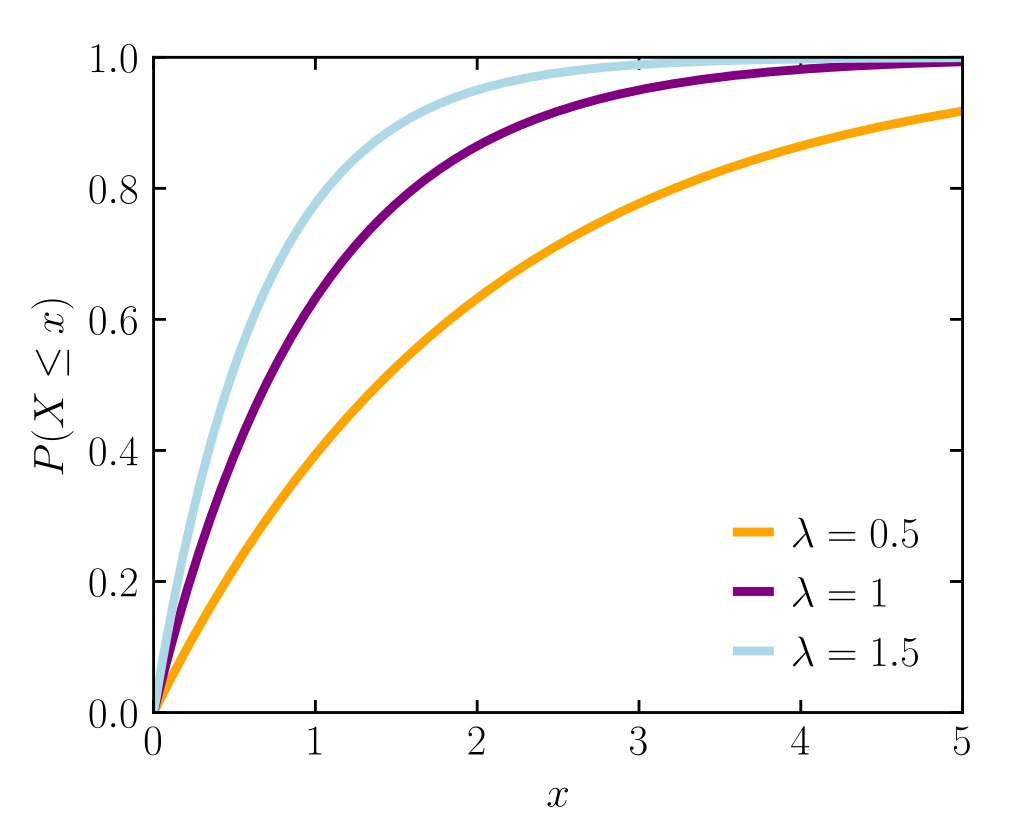
\includegraphics[width=0.7\linewidth]{images/countermeasures/cumulative_distribution_function.png}
    \caption{CDF of the exponential distribution}
    \label{fig:cdf}
\end{figure}
\vspace{3mm}

Going into the details, the Probability Density Function (PDF) of the exponential distribution is:
\[\ f(x, \lambda ) = \lambda e^{-\lambda x}, x \geq 0, \lambda \geq 0 \]
while the Cumulative Distribution Function (CDF), shown in Figure \ref{fig:cdf} is defined as follows:
\[\ F(x) = 1 - e^{-\lambda x} \]
By solving \(\ p = F(x) \), we obtain the inverse function
\[\ x = F^{-1}(p) = -\frac{1}{\lambda}\ln(1-p) \]
The idea is illustrated in Figure \ref{fig:distribution}. Random numbers are generated from a uniform distribution between \(\ 0 \) and \(\ 1 \). Each of the points is mapped according to \(\ x = F_{-1}(y) \). We can observe that using this strategy, most of the points end up close to 0, while only a few of them end up having high values.

\vspace{3mm}
\begin{figure}[H]
    \centering
    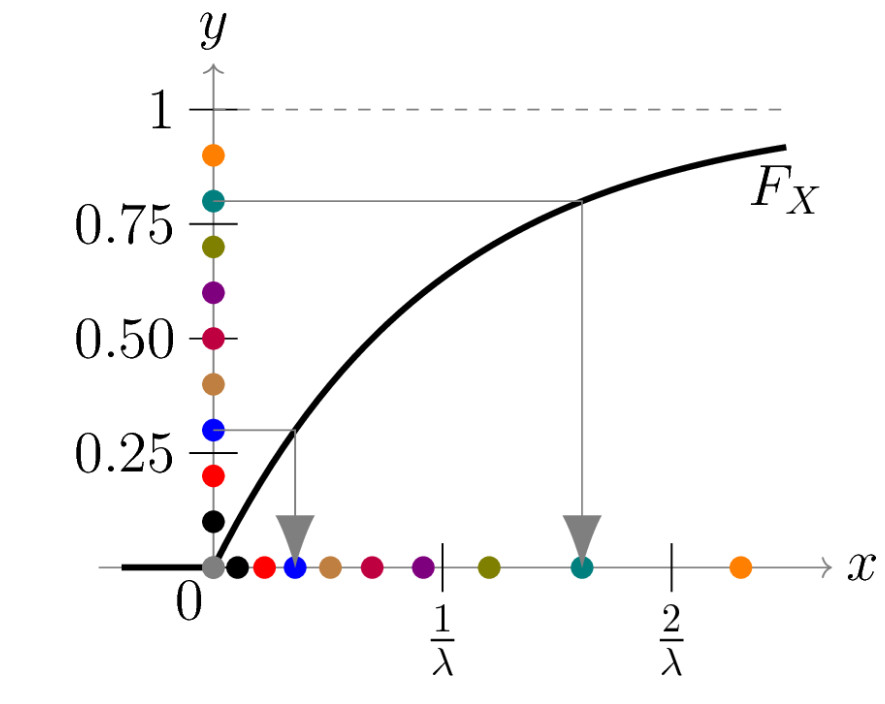
\includegraphics[width=0.7\linewidth]{images/countermeasures/inverse_transformation_method_for_exponential_distribution.jpg}
    \caption{Inverse transformation method for exponential distribution}
    \label{fig:distribution}
\end{figure}
\vspace{3mm}